%%
%% This is file `example_DarkConsole.tex',
%% generated with the docstrip utility.
%%
%% The original source files were:
%%
%% examples_kmbeamer.dtx  (with options: `DarkConsole')
%% Copyright (c) 2011-2016 Kazuki Maeda <kmaeda@kmaeda.net>
%% 
%% Distributable under the MIT License:
%% http://www.opensource.org/licenses/mit-license.php
%% 

\documentclass{beamer}

\usepackage{lipsum}             % for dummy text
\usepackage{stix}               % use the STIX font
\usepackage{hyperref}
\usepackage{color}
\usepackage{graphicx}
%% \usepackage{wrapfig}
\usepackage{array} % needed for \arraybackslash
\usepackage{graphicx}
\usepackage{adjustbox} % for \adjincludegraphics
\usepackage[ruled,vlined,linesnumbered]{algorithm2e}
\usepackage{listings}
\lstset{numbers=left, numbersep=1pt, xleftmargin=0.8em,frame=none,framexleftmargin=1em}
\usepackage{booktabs}
\usepackage{multirow}


\graphicspath{ {./} }

\usetheme{DarkConsole}

\title{15 minutes talk.}
\subtitle{Algorithms and Data Structures.}
\subtitle{Hashtable.}
\author{Konstantin Pachuev.}

\begin{document}

\begin{frame}
  \maketitle
\end{frame}

\begin{frame}{Outline}
  \tableofcontents
\end{frame}

\section{Statement.}

\begin{frame}{Statement of Work}
  Implement your own Hastable<K, V> class without using any library classes that are already
  available for the language or platform you are using to implement the hashtable.
  E.g., implement the hashtable using just simple arrays. The hashtable should support methods
  to add and remove elements. You are free to choose either hashing with chaining or hashing
  with open addressing for your implementation. Please also provide tests. Tell us the runtime
  of each class method using the O calculus.\footnote{\url{https://www.esrlabs.com/coding-assignments/}}
\end{frame}

\begin{frame}[allowframebreaks]{Requirements.}
  \begin{enumerate}

  \item \textcolor{yellow}{User's.}
    \begin{enumerate}
    \item Hashtable must store elements, provide insertion, retrieval and deletion of elements with basic
      or user defined types of keys and values.
    \item Hashtable should provide unified interface for user defined hash function.
    \end{enumerate}

  \item \textcolor{yellow}{Functional.}
    \begin{enumerate}
    \item Isertion must add an element to Hashtable or do nothing if element with such key is in Hashtable. 
    \item Deletion must remove element from Hashtable or do nothing if Hashtable doesn't contain element with such key.
    \item Retrieval must provide access to element's value or notify user if Hashtable doesn't contain element with such key.
    \item Notification must be delivered to user if user's hash function doesn't work properly.
    \end{enumerate}
    \framebreak
  \item \textcolor{yellow}{Performance.}
    \begin{enumerate}
    \item Performance of insertion, retrieval and deletion must at least be comparable with a well-known implementetion.
    \end{enumerate}

  \item \textcolor{yellow}{Implementation.}
    \begin{enumerate}
    \item Hashtable must be implemented as a class using simple arrays.
    \item Colision resolution strategy must be implemented with a separate
      chaining method or an open addressing method.
    \end{enumerate}

  \item \textcolor{yellow}{Delivery.}
    \begin{enumerate}
    \item Testing capabilities must be provided. 
    \item Runtime analysis must be delivered.
    \end{enumerate}
  \end{enumerate}
   
\end{frame}


\begin{frame}[allowframebreaks]{Specification.}
  \begin{enumerate}
  \item Implement Hashtable<K, V> as a C++ template class.
  \item Impletent hash functions for following C++ built in types \\
    int, char, bool and std::string type.
  \item Implement following required methods
  \begin{enumerate}
    \item Hashtable<K, V>::add(const K\& key, const V\& value)
    \item const V* Hashtable<K, V>::get(const K\& key)
    \item void Hashtable<K, V>::remove(const K\& key)
  \end{enumerate}
  \item Each required method must run in O(1) average case and O(n) in worst case.
  \item Throw an exception if user's hash function doesn't work properly. 
    \framebreak
  \item Implement correctness tests for int, char, bool and std::string types.
  \item Implement performance test for int and std::string types. 
  \item Implement corrctness test for user's difined key, value and hash function.
  \item All test should be implemented without using test frameworks.

  \end{enumerate}

\end{frame}

\section{Structure.}
\begin{frame}{Structure.}{Consept.}
  Hash Table uses separate chaining with linked lists method to resolve collisions
  \footnote{Different keys are assigned to the same bucket.}.
  
  \begin{itemize}
  \item Hashtable<K, V> consists of an array of buckets\footnote{Bucket and chain can be used interchangeably, a bucket is implemented as a linked list.}.
  \item A bucket is an object of LinkedList<K, V> class.
  \item LinkedList<K, V> class is an implementation of singly linked list customized to store values with unique keys.
  \end{itemize}
\end{frame}

\begin{frame}{Structure.}{Classes.}
  \begin{itemize}
  \item namespace esr
    \begin{itemize}
      \item class Hashtable<K, V>
        \begin{itemize}
          \item class iterator
        \end{itemize}
      \item class linkedlist<K, V>
      \item class listnode<K, V>
      \item class hasher<K>
      \item class hash\_function<K>
      \item class hash\_function<int>
      \item class hash\_function<char>
      \item class hash\_function<bool>
      \item class hash\_function<std::string>
      \item namespace exception
        \begin{itemize}
          \item class hashtable
          \item class bucket\_index 
          \item class end\_iterator
        \end{itemize}
    \end{itemize}
  \end{itemize}
\end{frame}


\begin{frame}{Structure.}{Classes from esr namespace.}
    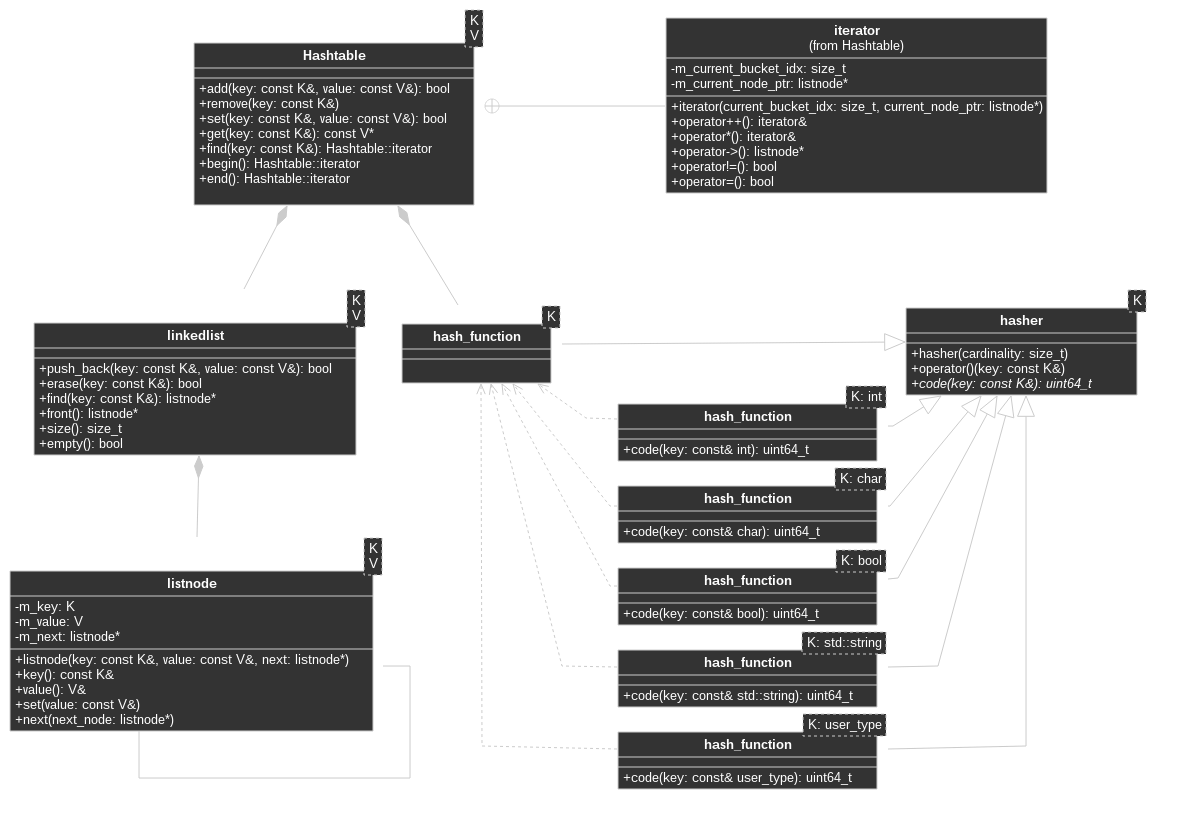
\includegraphics[scale=0.3]{structure_classes}
\end{frame}

\begin{frame}{Structure.}{Classes from esr::exception namespace.}
  \begin{figure}
    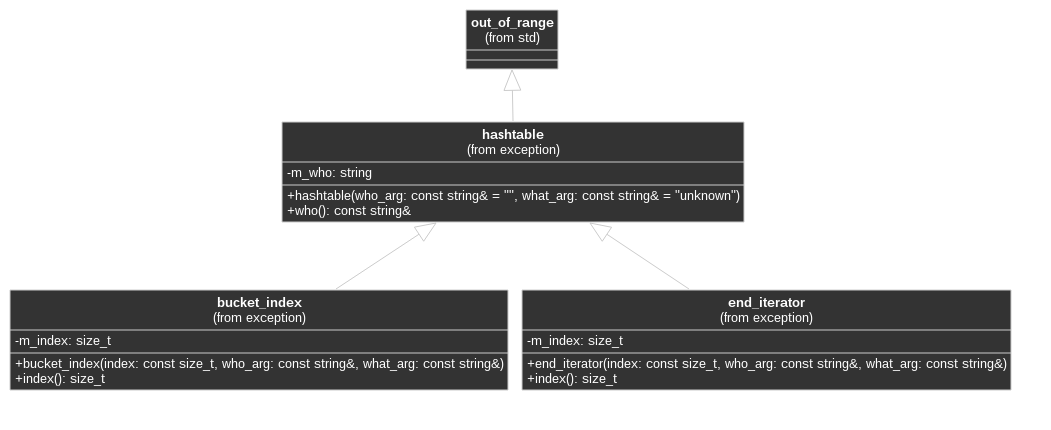
\includegraphics[scale=0.3]{structure_exceptions_classes}
  \end{figure}
\end{frame}


\begin{frame}{Structure.}{Insertion.}
  \begin{figure}
    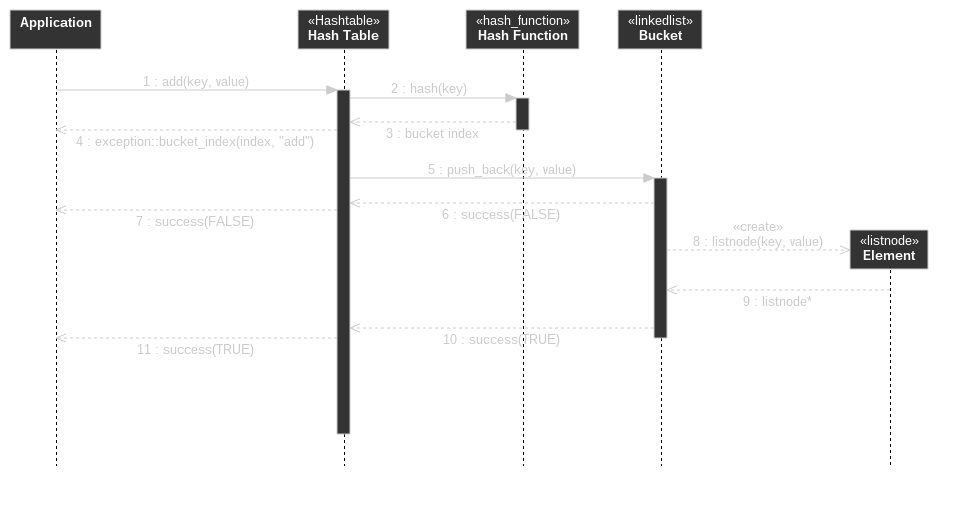
\includegraphics[scale=0.3]{structure_insertion_sequence}
  \end{figure}
\end{frame}

\begin{frame}{Structure.}{Deletion.}
  \begin{figure}
    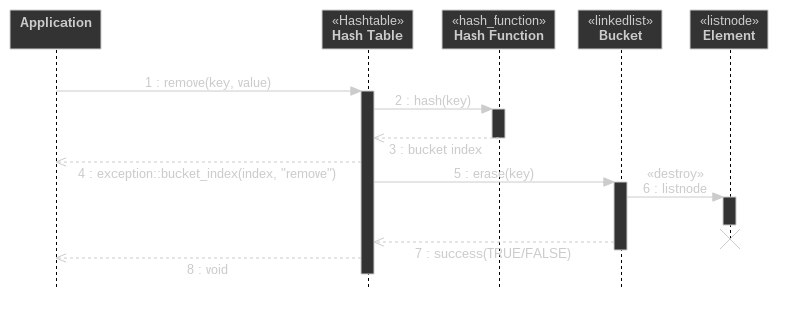
\includegraphics[scale=0.3]{structure_deletion_sequence}
  \end{figure}
\end{frame}

\begin{frame}{Structure.}{Set.}
  \begin{figure}
    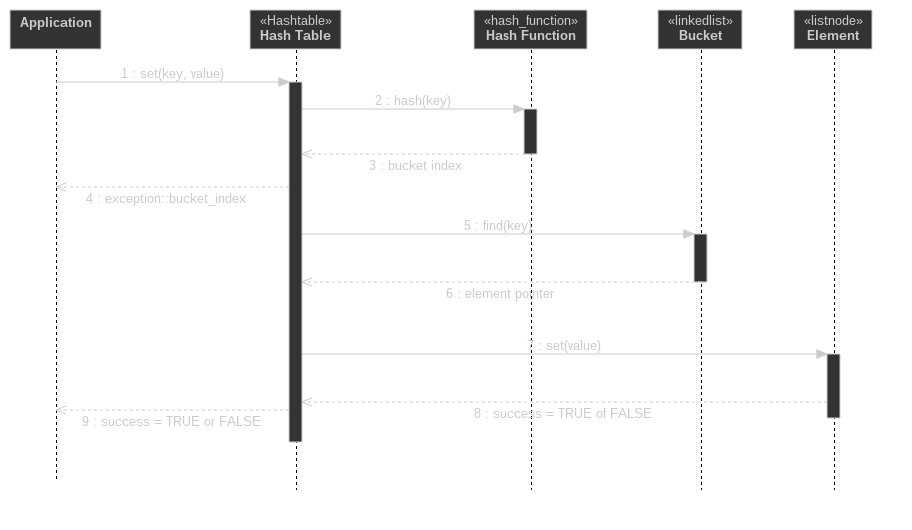
\includegraphics[scale=0.3]{structure_set_sequence}
  \end{figure}
\end{frame}

\begin{frame}{Structure.}{Get.}
  \begin{figure}
    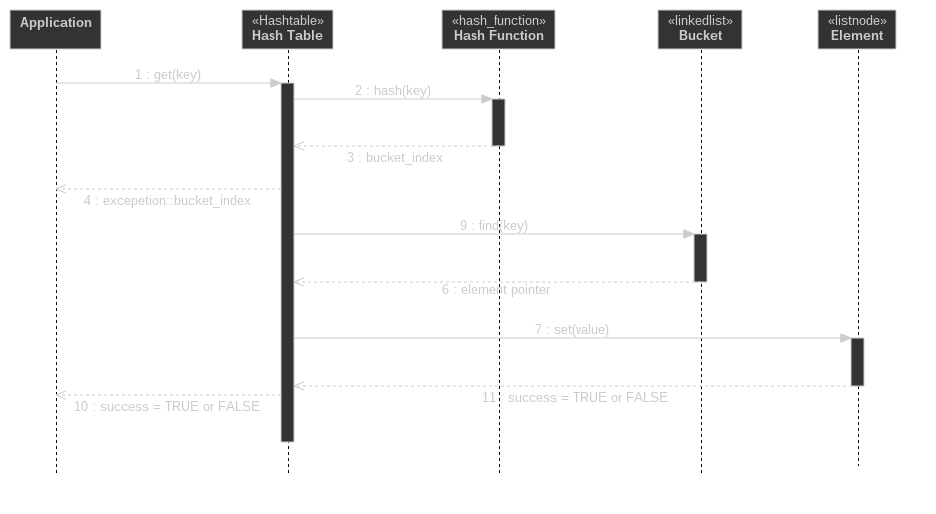
\includegraphics[scale=0.3]{structure_get_sequence}
  \end{figure}
\end{frame}

\begin{frame}{Structure.}{Find.}
  \begin{figure}
    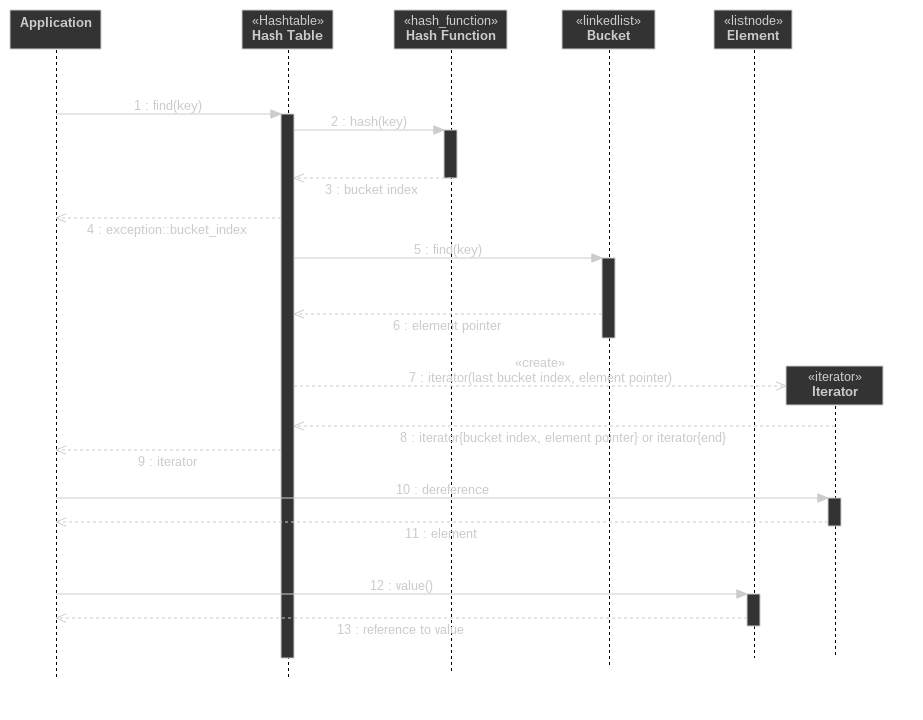
\includegraphics[scale=0.3]{structure_find_sequence}
  \end{figure}
\end{frame}





\section{Implementation.}

\begin{frame}{Implementation.}{Load Factor.}
  An Insertion, Deletion or Retrieval operation consists of the following steps.
  \begin{enumerate}
  \item Obtaining bucket index in bucket array using a hash function which maps key to bucket index.
    Running time is O(1).
  \item Finding an element of bucket, scaning a linked list and comparing the keys.
    Running time is O(size), size is a number of elements in list. 
    \item Performing a required operation. Running time is O(1).
  \end{enumerate}
  %%To perform one of Insertion, Deletion or Retrieval operations we need
  %%Among these three steps only search for element in bucket
  %%depends on number of elements, because it scans the list. So to achieve O(1) performance
  %%we should keep the size of the list near some constant value.

  \par The average number of elements stored in bucket is
  \begin{equation}
    \alpha = \frac{n}{m},
  \end{equation}
  which is a Load Factor for Hashtable with m buckets that stores n elements.
\end{frame}

%%\begin{frame}{Implementation.}{Insertion.}
%%  \begin{figure}
%%    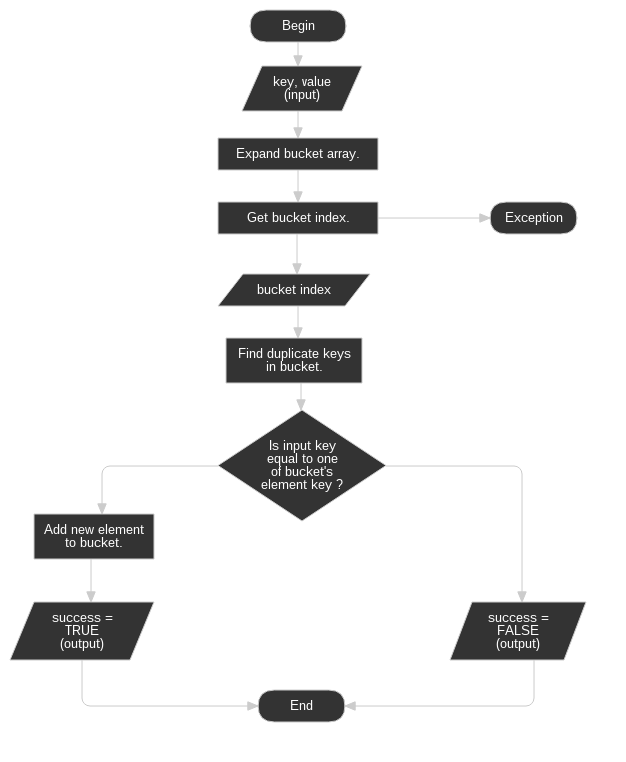
\includegraphics[scale=0.3]{implementation_insertion_flowchart}
%%  \end{figure}
%%\end{frame}

\begin{frame}[allowframebreaks]{Implementation.}{Insertion.}
  \IncMargin{1em}
  \resizebox{!}{43mm}{\begin{algorithm}[H]
      \caption{add(key, value)}
      \SetFuncSty{textsc}
      \SetDataSty{emph}
      %%\newcommand{\expr}[1]{$\langle${#1}$\rangle$}
      %%\newcommand{\commentsty}[1]{{\color{DarkGreen}#1}}
      \SetCommentSty{commentsty}

      \DontPrintSemicolon
      \scriptsize
      \SetAlgoLined
      \SetKwData{key}{key}
      \SetKwData{value}{value}
      \SetKwInOut{Input}{input}
      \SetKwInOut{Output}{output}
      \SetKwInOut{Parameter}{parameter}
      \SetKwData{success}{success}
      \SetKwData{bucketIndex}{bucketIndex}
      \SetKwData{loadFactorBoundUp}{loadFactorBoundUp}
      \SetKwData{bucketsCount}{bucketsCount}
      \SetKwData{elementsCount}{elementsCount}
      \SetKwData{bucket}{bucket}
      \SetKwData{bucketArray}{bucketArray}
      \SetKwData{loadFactor}{loadFactor}
      \SetKwFunction{Hash}{Hash}
      \SetKwFunction{Exception}{Exception}
      \SetKwFunction{AddElementToBucket}{AddElementToBucket}
      \SetKwFunction{Resize}{Resize}
      \SetKwArray{Array}{array}
      \SetKwFunction{A}{Hash}
 
      \Input{\key,\value}
      \Output{\success}
      \Parameter{\elementsCount, \bucketsCount, \loadFactorBoundUp,\\
        \bucketArray is an \Array[ 0..\bucketsCount] of buckets }
      \everypar={\nl}
      \If{\elementsCount $=$ 0}{
        \Resize{1}
      }
      \loadFactor$\leftarrow$ \( \frac{\elementsCount}{\bucketsCount}\) \;
      \If{\loadFactor $>$ \loadFactorBoundUp}{
        \Resize{2$\cdot$\bucketsCount}
      }
      \bucketIndex$\leftarrow$ \Hash{$Key$}\;
      \If{\bucketIndex $\geq$ \bucketsCount}{
        \Exception{\bucketIndex}
      }
      \bucket$\leftarrow$ \bucketArray[\bucketIndex]\;
      \success$\leftarrow$ \bucket.\AddElementToBucket{\key,\value}\;
      \If{\success = TRUE}{\bucketsCount $\leftarrow$ \bucketsCount + 1\;}
      \KwRet{\success}
  \end{algorithm}}
  \framebreak
 \resizebox{!}{43mm}{\begin{algorithm}[H]
      \caption{AddElementToBucket(key, value)}
      \SetFuncSty{textsc}
      \SetDataSty{emph}
      \SetCommentSty{commentsty}
      \DontPrintSemicolon
      \scriptsize
      \SetAlgoLined
      \SetKwData{key}{key}
      \SetKwData{value}{value}
      \SetKwInOut{Input}{input}
      \SetKwInOut{Output}{output}
      \SetKwInOut{Parameter}{parameter}
      \SetKwData{success}{success}
      \SetKwData{front}{front}
      \SetKwData{nodesCount}{nodesCount}
      \SetKwData{node}{node}
      \SetKwComment{Comment}{$\triangleright$ }{}
      \Input{\key,\value}
      \Output{\success}
      \Parameter{\front, \nodesCount}
      \everypar={\nl}
      \eIf{\front $=$ NULL} {
        \front $\gets$ $\langle$ Create new list node with input \key, \value$\rangle$\;
      }{
        \ForEach{node $n$ of list} { 
          \If{n.key $=$ key} {
            \KwRet FALSE
          }
        }
        \node $\gets$ $\langle$ Create new list node with input \key, \value$\rangle$\; 
        \node.next $\gets$ \front \;
        \front $\gets$ \node \; 
      }
      \nodesCount $\gets$ \nodesCount + 1\;
      \KwRet{TRUE}
  \end{algorithm}}

\end{frame}

\begin{frame}[allowframebreaks]{Implementation.}{Deletion.}
  \IncMargin{1em}
  \resizebox{!}{43mm}{\begin{algorithm}[H]
      \caption{remove(key)}
      \SetFuncSty{textsc}
      \SetDataSty{emph}
      \SetCommentSty{commentsty}

      \DontPrintSemicolon
      \scriptsize
      \SetAlgoLined
      \SetKwData{key}{key}
      \SetKwInOut{Input}{input}
      \SetKwInOut{Output}{output}
      \SetKwInOut{Parameter}{parameter}
      \SetKwData{success}{success}
      \SetKwData{bucketIndex}{bucketIndex}
      \SetKwData{loadFactorBoundLow}{loadFactorBoundLow}
      \SetKwData{bucketsCount}{bucketsCount}
      \SetKwData{elementsCount}{elementsCount}
      \SetKwData{bucket}{bucket}
      \SetKwData{bucketArray}{bucketArray}
      \SetKwData{loadFactor}{loadFactor}
      \SetKwFunction{Hash}{Hash}
      \SetKwFunction{Exception}{Exception}
      \SetKwFunction{RemoveElementFromBucket}{RemoveElementFromBucket}
      \SetKwFunction{Resize}{Resize}
      \SetKwArray{Array}{array}
      \SetKwFunction{A}{Hash}
 
      \Input{\key}
      \Parameter{\elementsCount, \bucketsCount, \loadFactorBoundLow,\\
        \bucketArray is an \Array[ 0..\bucketsCount] of buckets }
      \everypar={\nl}
      \If{\elementsCount $=$ 0}{
        \KwRet
      }
      \bucketIndex$\gets$ \Hash{$Key$}\;
      \If{\bucketIndex $\geq$ \bucketsCount}{
        \Exception{\bucketIndex}
      }
      \bucket$\gets$ \bucketArray[\bucketIndex]\;
      \success$\gets$ \bucket.\RemoveElementFromBucket{\key}\;
      \If{\success $=$ FALSE}{
        \KwRet
      }
      \elementsCount$\gets$ \elementsCount  - 1 \;
      \If{\elementsCount $=$ 0} {
        \Resize{0}\;
        \KwRet
      }

      \loadFactor$\leftarrow$ \( \frac{\elementsCount}{\bucketsCount}\) \;
      \If{\loadFactor $<$ \loadFactorBoundLow}{
        \Resize{\(\frac{\bucketsCount}{2}\)}
      }

      
  \end{algorithm}}
 
  \framebreak

  \resizebox{!}{43mm}{\begin{algorithm}[H]
      \caption{RemoveElementFromBucket(key)}
      \SetFuncSty{textsc}
      \SetDataSty{emph}
      \SetCommentSty{commentsty}
      \DontPrintSemicolon
      \scriptsize
      \SetAlgoLined
      \SetKwData{key}{key}
      \SetKwData{value}{value}
      \SetKwInOut{Input}{input}
      \SetKwInOut{Output}{output}
      \SetKwInOut{Parameter}{parameter}
      \SetKwData{success}{success}
      \SetKwData{front}{front}
      \SetKwData{nodesCount}{nodesCount}
      \SetKwData{node}{node}
      \SetKwData{prev}{prev}
      \SetKwComment{Comment}{$\triangleright$ }{}
      \Input{\key,\value}
      \Output{\success}
      \Parameter{\front, \nodesCount}
      \everypar={\nl}
      \prev $\gets$ NULL \;
      \ForEach{node $n$ of list} { 
        \If{n.key $=$ key} {
          \eIf{n $=$ front}{
            \front $\gets$ n.next \;
          }{
            \prev.next $\gets$ n.next \;
          }
          $\langle$ Delete list node $n$ $\rangle$\;
          \nodesCount $\gets$ \nodesCount - 1 \;
          \KwRet TRUE 
        }
        \prev $\gets$ n \;
      }
      \KwRet FALSE
  \end{algorithm}}

  %%\begin{figure}
  %%  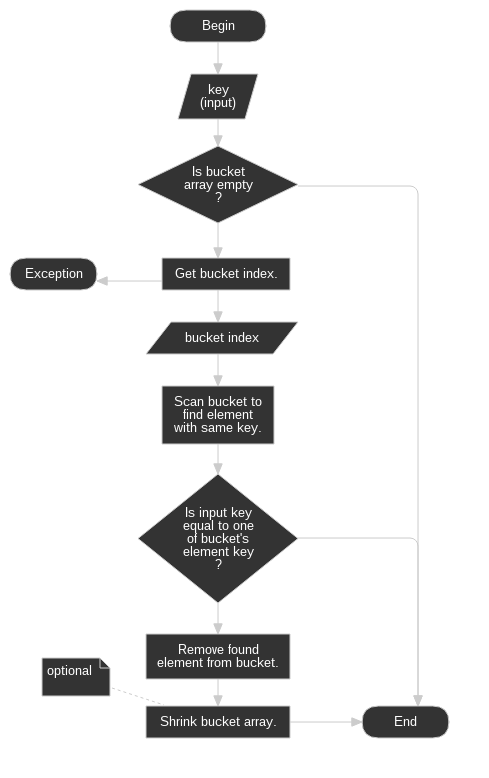
\includegraphics[scale=0.3]{implementation_deletion_flowchart}
  %% \end{figure}
\end{frame}

\begin{frame}{Implementation.}{Resizing.}
  \IncMargin{1em}
  \resizebox{!}{43mm}{\begin{algorithm}[H]
      \caption{resize(newBucketsCount)}
      \SetFuncSty{textsc}
      \SetDataSty{emph}
      \SetCommentSty{commentsty}

      \DontPrintSemicolon
      \scriptsize
      \SetAlgoLined
      \SetKwData{key}{key}
      \SetKwInOut{Input}{input}
      \SetKwInOut{Output}{output}
      \SetKwInOut{Parameter}{parameter}
      \SetKwData{success}{success}
      \SetKwData{bucketIndex}{bucketIndex}
      \SetKwData{loadFactorBoundLow}{loadFactorBoundLow}
      \SetKwData{bucketsCount}{bucketsCount}
      \SetKwData{newBucketsCount}{newBucketsCount}
      \SetKwData{elementsCount}{elementsCount}
      \SetKwData{bucket}{bucket}
      \SetKwData{bucketArray}{bucketArray}
      \SetKwData{newBucketArray}{newBucketArray}
      \SetKwData{loadFactor}{loadFactor}
      \SetKwData{element}{element}
      \SetKwFunction{Hash}{Hash}
      \SetKwFunction{Exception}{Exception}
      \SetKwFunction{AddElementToBucket}{AddElementToBucket}
      \SetKwFunction{Resize}{Resize}
      \SetKwArray{Array}{array}
      \SetKwFunction{A}{Hash}
 
      \Input{\newBucketsCount}
      \Parameter{\bucketsCount, \\
        \bucketArray is an \Array[ 0..\bucketsCount] of buckets }
      \everypar={\nl}
      \newBucketArray$\gets$ NULL \;
      \If{\newBucketsCount$\neq$ 0}{
        \newBucketArray$\gets$ $\langle$ Create \Array{0..\newBucketsCount}$\rangle$\;
        \Hash$\gets$ $\langle$Create new Hash Function from it's family$\rangle$\;
      }

      \ForEach{\bucket of \bucketArray} { 
        \ForEach{\element of \bucket} {
          \bucketIndex$\gets$ \Hash{element.key} \;
          \If{\bucketIndex $\geq$ \bucketsCount}{
            $\langle$throw out of range exception$\rangle$\;
            \success$\gets$ \bucket.\AddElementToBucket{\element.key,\element.value} \; 
            \newBucketsCount$\gets$ \newBucketsCount + 1 \;
          }
        }
      }
      \If{\bucketArray not empty} {
        $\langle$Delete \bucketArray$\rangle$\;
      }
      \elementsCount$\gets$ \elementsCount \;
      \bucketsCount$\gets$ \newBucketsCount \;
      \bucketArray$\gets$ \newBucketArray \;
  \end{algorithm}}

  %%\begin{figure}
  %%  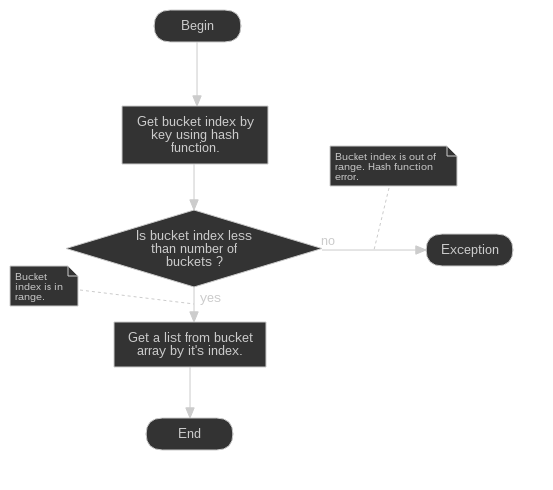
\includegraphics[scale=0.3]{implementation_index_flowchart}
  %%\end{figure}
\end{frame}

%%\begin{frame}{Implementation.}{Expand/Shrink by Resizing.}
%%  \begin{figure}
%%    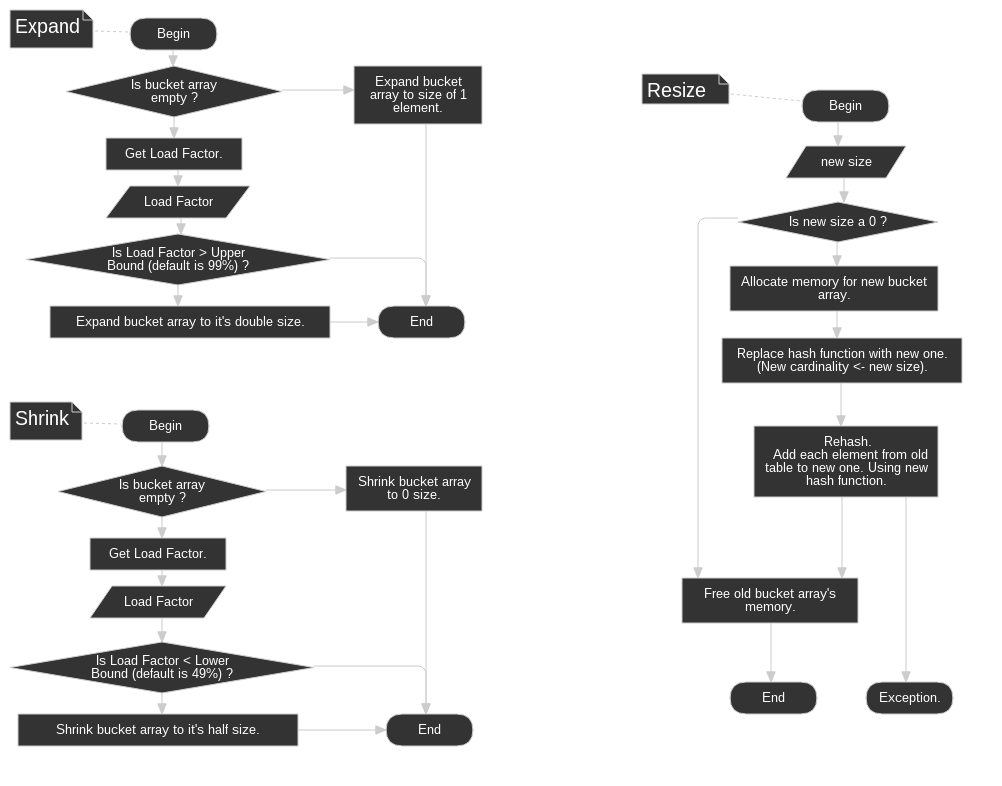
\includegraphics[scale=0.3]{implementation_resize_flowchart}
%%  \end{figure}
%%\end{frame}

\begin{frame}{Implementation.}{Iterator.}
  \vspace*{10pt}
  Iterator's position is defined by pair which is
  \begin{itemize}
    \item a \textit{bucket index}, index of linked list in an array;
    \item an \textit{element pointer}, pointer to node of linked list.
  \end{itemize}

  \begin{tabular}{p{.4\textwidth} p{.5\textwidth}}
    \adjincludegraphics[width=1.5\linewidth,valign=t]{iterator} &
    \raggedright{
      \vspace*{10pt}
      Array of N buckets
      \begin{itemize}
      \item Empty buckets
        \begin{itemize}
        \item from \textbf{\textit{L\textsubscript{0}}} to \textbf{\textit{L\textsubscript{i-1}}}
        \item from \textbf{\textit{L\textsubscript{j+1}}} to \textbf{\textit{L\textsubscript{k-1}}}
        \item from \textbf{\textit{L\textsubscript{k+1}}} to \textbf{\textit{L\textsubscript{n}}}
        \end{itemize}
      \item Iterators
        \begin{itemize}
        \item \textbf{\textit{b}} is a begin iterator 
        \item \textbf{\textit{e}} is an end iterator 
        \item \textbf{\textit{n\textsubscript{2}}} is next to n1 
        \item \textbf{\textit{m\textsubscript{2}}} is next to \textbf{\textit{m\textsubscript{1}}} 
        \end{itemize}
      \end{itemize}
    }
  \end{tabular}
\end{frame}

\begin{frame}{Implementation.}{Iterator Begin, End, Current.}
  \begin{itemize}
  \item Begin Iterator
    \begin{itemize}
    \item \{first not empty bucket index, pointer to first element\} 
    \end{itemize}
  \item End Iterator
    \begin{itemize}
    \item \{last bucket index, NULL\} 
    \end{itemize}
  \item Current Iterator
    \begin{itemize}
    \item \{current bucket index, current element pointer\} 
    \end{itemize}
  \end{itemize}
  %%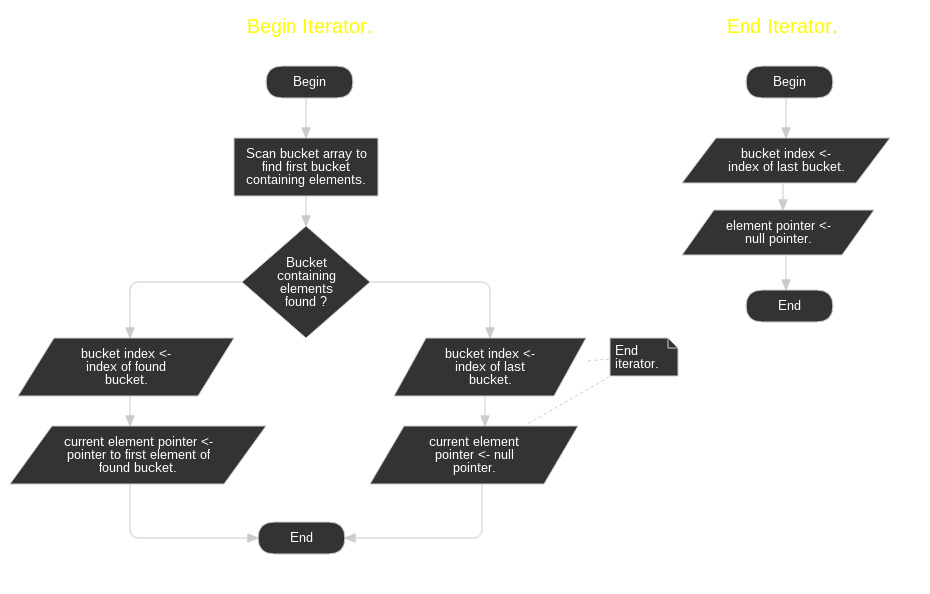
\includegraphics[scale=0.35]{implementation_begin_iterator_flowchart}
  \IncMargin{1em}
  \resizebox{!}{28mm}{\begin{algorithm}[H]
      \caption{Begin()}
      \SetFuncSty{textsc}
      \SetDataSty{emph}
      \SetCommentSty{commentsty}

      \DontPrintSemicolon
      \scriptsize
      \SetAlgoLined
      \SetKwData{key}{key}
      \SetKwInOut{Input}{input}
      \SetKwInOut{Output}{output}
      \SetKwInOut{Parameter}{parameter}
      \SetKwData{success}{success}
      \SetKwData{bucketIndex}{bucketIndex}
      \SetKwData{loadFactorBoundLow}{loadFactorBoundLow}
      \SetKwData{bucketsCount}{bucketsCount}
      \SetKwData{newBucketsCount}{newBucketsCount}
      \SetKwData{elementsCount}{elementsCount}
      \SetKwData{bucket}{bucket}
      \SetKwData{bucketArray}{bucketArray}
      \SetKwData{newBucketArray}{newBucketArray}
      \SetKwData{loadFactor}{loadFactor}
      \SetKwData{firstNotEmptyBucketIndex}{firstNotEmptyBucketIndex}
      \SetKwData{element}{element}
      \SetKwFunction{Hash}{Hash}
      \SetKwFunction{Exception}{Exception}
      \SetKwFunction{AddElementToBucket}{AddElementToBucket}
      \SetKwFunction{Resize}{Resize}
      \SetKwArray{Array}{array}
      \SetKwFunction{A}{Hash}
 
      \Parameter{\bucketsCount, \\
        \bucketArray is an \Array[ 0..\bucketsCount] of buckets }
      \everypar={\nl}
      \firstNotEmptyBucketIndex$\gets$ 0 \;
      \While{\firstNotEmptyBucketIndex $<$ \bucketsCount} {
        \If{\bucketArray[\firstNotEmptyBucketIndex] is not empty}{
          break\;
        }
        \firstNotEmptyBucketIndex$\gets$ \firstNotEmptyBucketIndex + 1\;
      }
      \If{\firstNotEmptyBucketIndex $=$ \bucketsCount}{
        \KwRet $\langle$End Iterator$\rangle$\;
      }
      \bucket$\gets$ \bucketArray[\firstNotEmptyBucketIndex]\;
      \KwRet $\langle$Begin Iterator$\rangle$\;
  \end{algorithm}}
\end{frame}

\begin{frame}{Implementation.}{Iterator Advance.}
  \IncMargin{1em}
  \resizebox{!}{43mm}{\begin{algorithm}[H]
      \caption{Advance()}
      \SetFuncSty{textsc}
      \SetDataSty{emph}
      \SetCommentSty{commentsty}

      \DontPrintSemicolon
      \scriptsize
      \SetAlgoLined
      \SetKwData{key}{key}
      \SetKwInOut{Input}{input}
      \SetKwInOut{Output}{output}
      \SetKwInOut{Parameter}{parameter}
      \SetKwData{success}{success}
      \SetKwData{bucketIndex}{bucketIndex}
      \SetKwData{loadFactorBoundLow}{loadFactorBoundLow}
      \SetKwData{bucketsCount}{bucketsCount}
      \SetKwData{newBucketsCount}{newBucketsCount}
      \SetKwData{elementsCount}{elementsCount}
      \SetKwData{bucket}{bucket}
      \SetKwData{bucketArray}{bucketArray}
      \SetKwData{newBucketArray}{newBucketArray}
      \SetKwData{loadFactor}{loadFactor}
      \SetKwData{nextBucketIndex}{nextBucketIndex}
      \SetKwData{nextNotEmptyBucketIndex}{nextNotEmptyBucketIndex}
      \SetKwData{element}{element}
      \SetKwData{elementPointer}{elementPointer}
      \SetKwFunction{Hash}{Hash}
      \SetKwFunction{Exception}{Exception}
      \SetKwFunction{AddElementToBucket}{AddElementToBucket}
      \SetKwFunction{Resize}{Resize}
      \SetKwArray{Array}{array}
      \SetKwFunction{A}{Hash}
 
      \Parameter{\bucketsCount, \bucketIndex, \elementPointer\\
        \bucketArray is an \Array[ 0..\bucketsCount] of buckets }
      \everypar={\nl}

      \elementPointer$\gets$ \elementPointer.next \;
      \If{\elementPointer $=$ NULL}{
        \nextBucketIndex$\gets$ \nextBucketIndex + 1 \;
        \For{i=\nextBucketIndex\emph{\KwTo} \bucketsCount}{
          \eIf{\bucketArray[\nextBucketIndex] is empty} {
            \nextBucketIndex$\gets$ \nextBucketIndex + 1\;
          }{
            break \;
          }
        }
        \nextNotEmptyBucketIndex$\gets$ \nextBucketIndex \;
        \eIf{\nextNotEmptyBucketIndex $<$ \bucketsCount}{
          \bucketIndex$\gets$ \nextNotEmptyBucketIndex \;
          \bucket$\gets$ \bucketArray[\bucketIndex] \;
          \elementPointer$\gets$ \bucket.front \;
        }{
          \bucketIndex$\gets$ \bucketsCount - 1 \;
          \elementPointer$\gets$ NULL \;
        }
      }
  \end{algorithm}}


  %%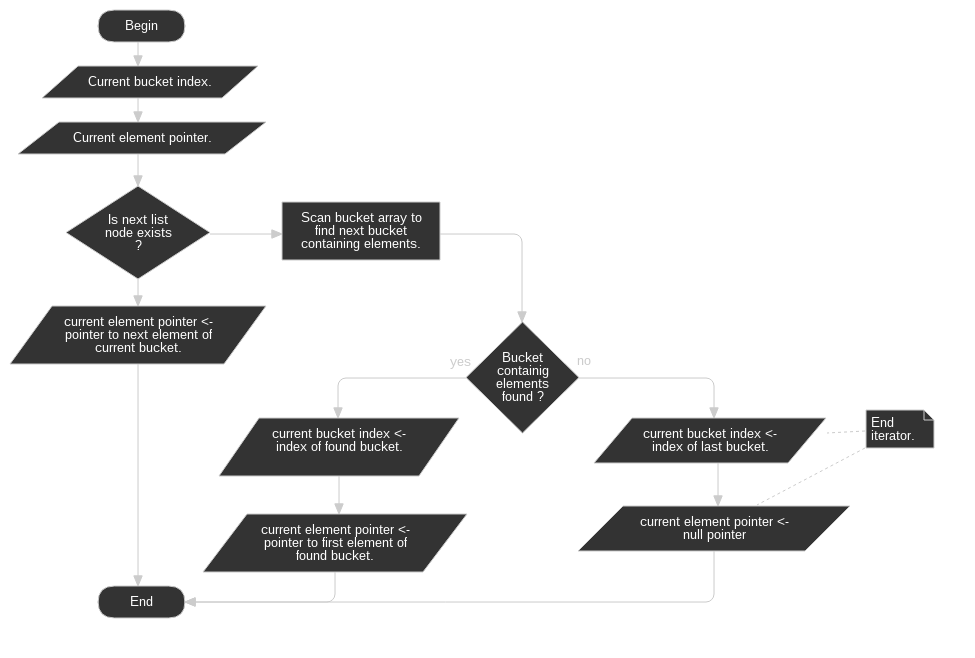
\includegraphics[scale=0.35]{implementation_advance_iterator_flowchart}
\end{frame}

\begin{frame}{Implementation.}{Set/Get/Find.}
  \begin{figure}
    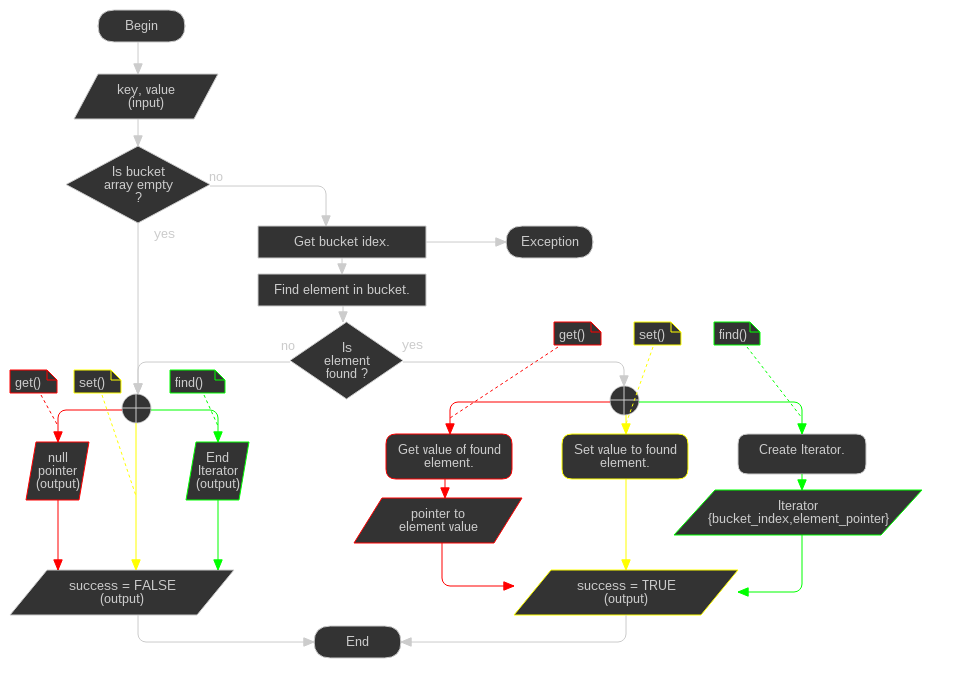
\includegraphics[scale=0.3]{implementation_set_get_find_flowchart}
  \end{figure}
\end{frame}

\begin{frame}{Tests.}
  \begin{enumerate}
  \item Correctnes tests.
    \begin{enumerate}
    \item Insertions and Retrievals.
    \item Copy and Assignments.
    \item Deletion.
    \end{enumerate}
  \item Performance tests.
    \begin{enumerate}
    \item Integer Keys Isertions and Retrievals.
    \item Fixed Length String Keys Isertions and Retrievals.
    \item Variable Length String Keys Isertions and Retrievals.
    \end{enumerate}
  \item Application Sample: user's hash function test.
  \end{enumerate}
\end{frame}

\begin{frame}{Tests.}{Correctness.}
  Tests functional correctness of Hashtable<K, V> for combinations of
  key type and value type, \textit{int, bool, std::string}. 
  \begin{enumerate}
    \item Isertion/Retrieval Tests (9*3*2 = 48 tests).   
      \begin{enumerate}
      \item add() positive/negative.
      \item get() positive/negative.
      \item find() positive/negative.
      \end{enumerate}
    \item Copy/Assignments Tests (9*2*1 = 18 tests). 
      \begin{enumerate}
      \item Copy Constructor.
      \item Assignment Operator.
      \end{enumerate}
    \item  Deletion Tests (9*1*2 = 18 tests).
      \begin{enumerate}
        \item remove() positive/negative. 
      \end{enumerate}
  \end{enumerate}
\end{frame}

\begin{frame}{Tests.}{Performance.}
  Tests performance of Hashtable<K, V> for \textit{int} and \textit{std::string}
  key types with \textit{int} value type.
  \begin{enumerate}
    \item Integer key test. Key length is 4 bytes. Doubles number of elements.
    \item Fixed Length string key test. Key length is 20 bytes. Doubles number of elements. 
    \item Variable Length string key test. Number of elements is 10000. Key length is 20 bytes. Doubles number of elements. 
  \end{enumerate}
\end{frame}



\begin{frame}{Tests.}{Performance. Integers.}
  \begin{figure}
    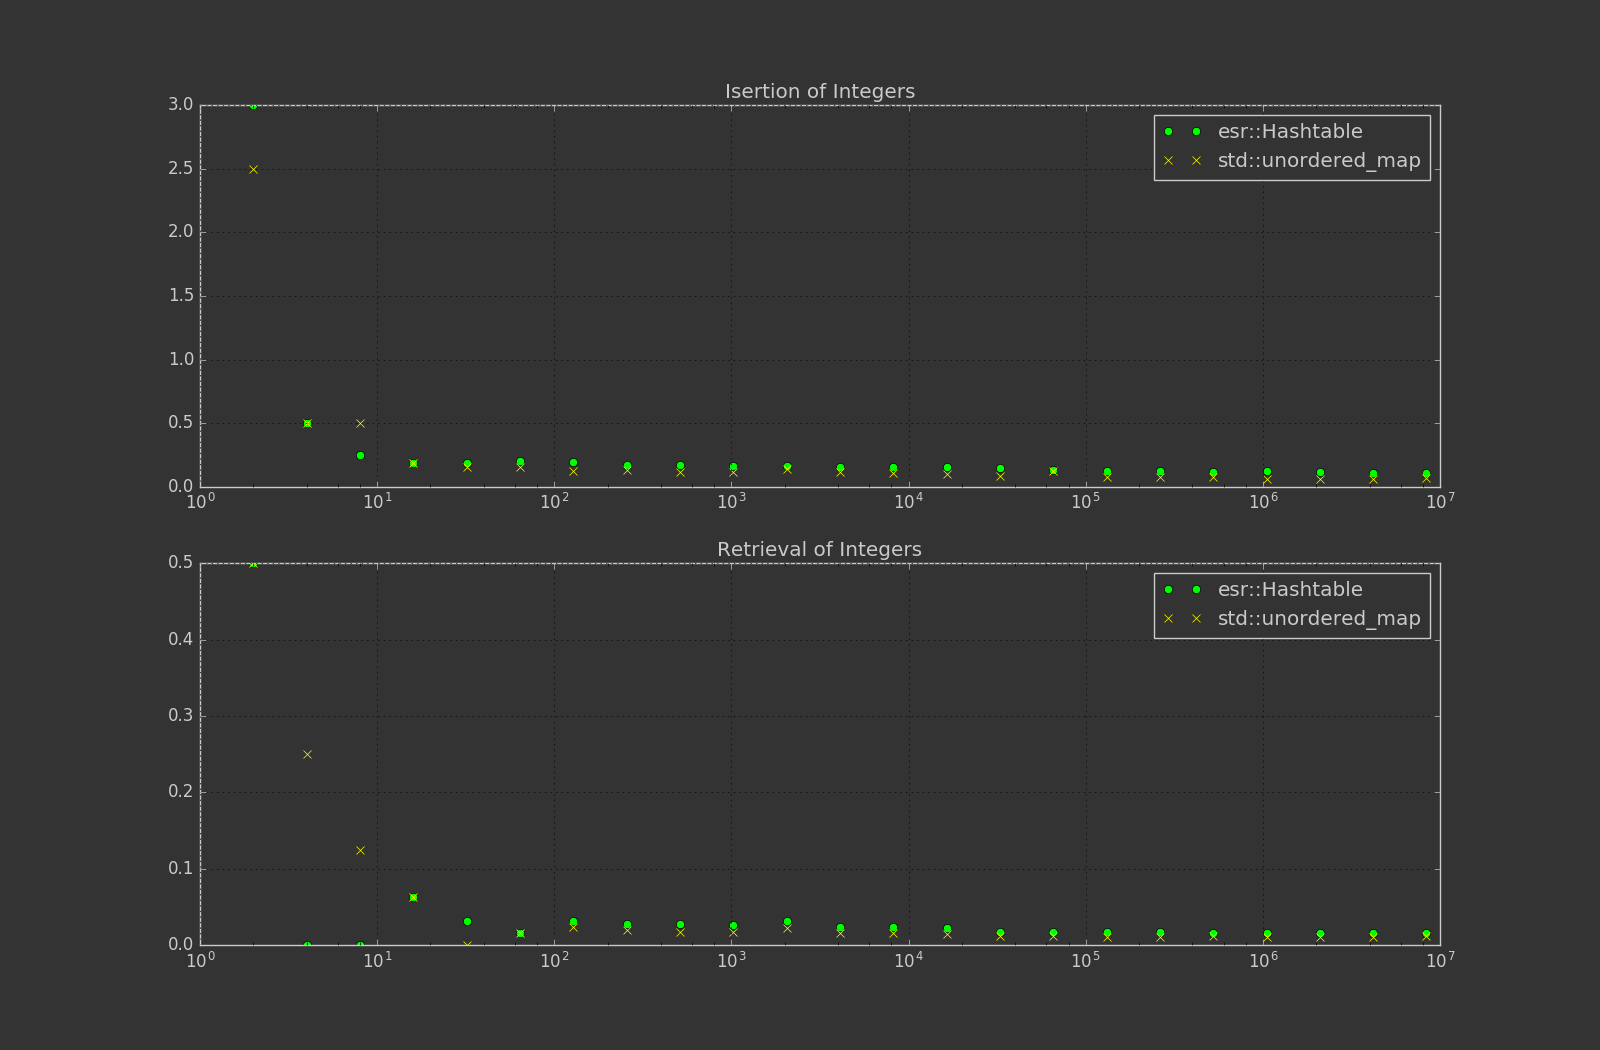
\includegraphics[scale=0.3]{int_perf}
  \end{figure}
\end{frame}

\begin{frame}{Tests.}{Performance. Fixed Length Strings.}
  \begin{figure}
    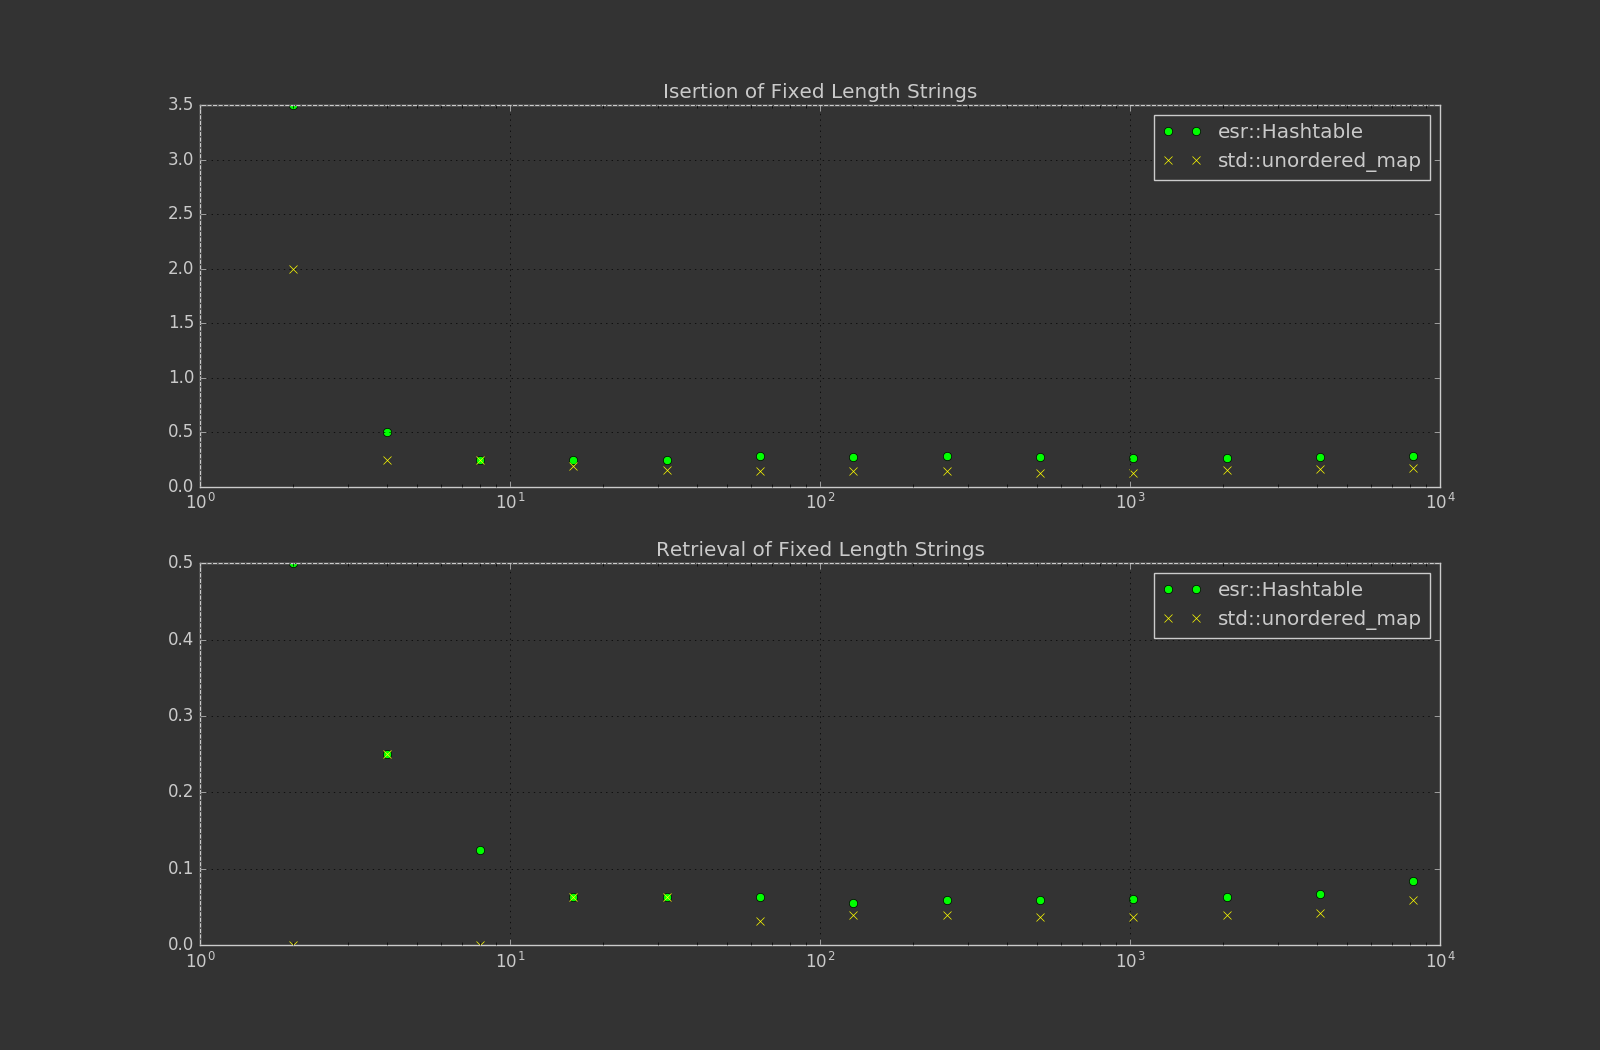
\includegraphics[scale=0.3]{fstr_perf}
  \end{figure}
\end{frame}

\begin{frame}{Tests.}{Performance. Variable Length Strings.}
  \begin{figure}
    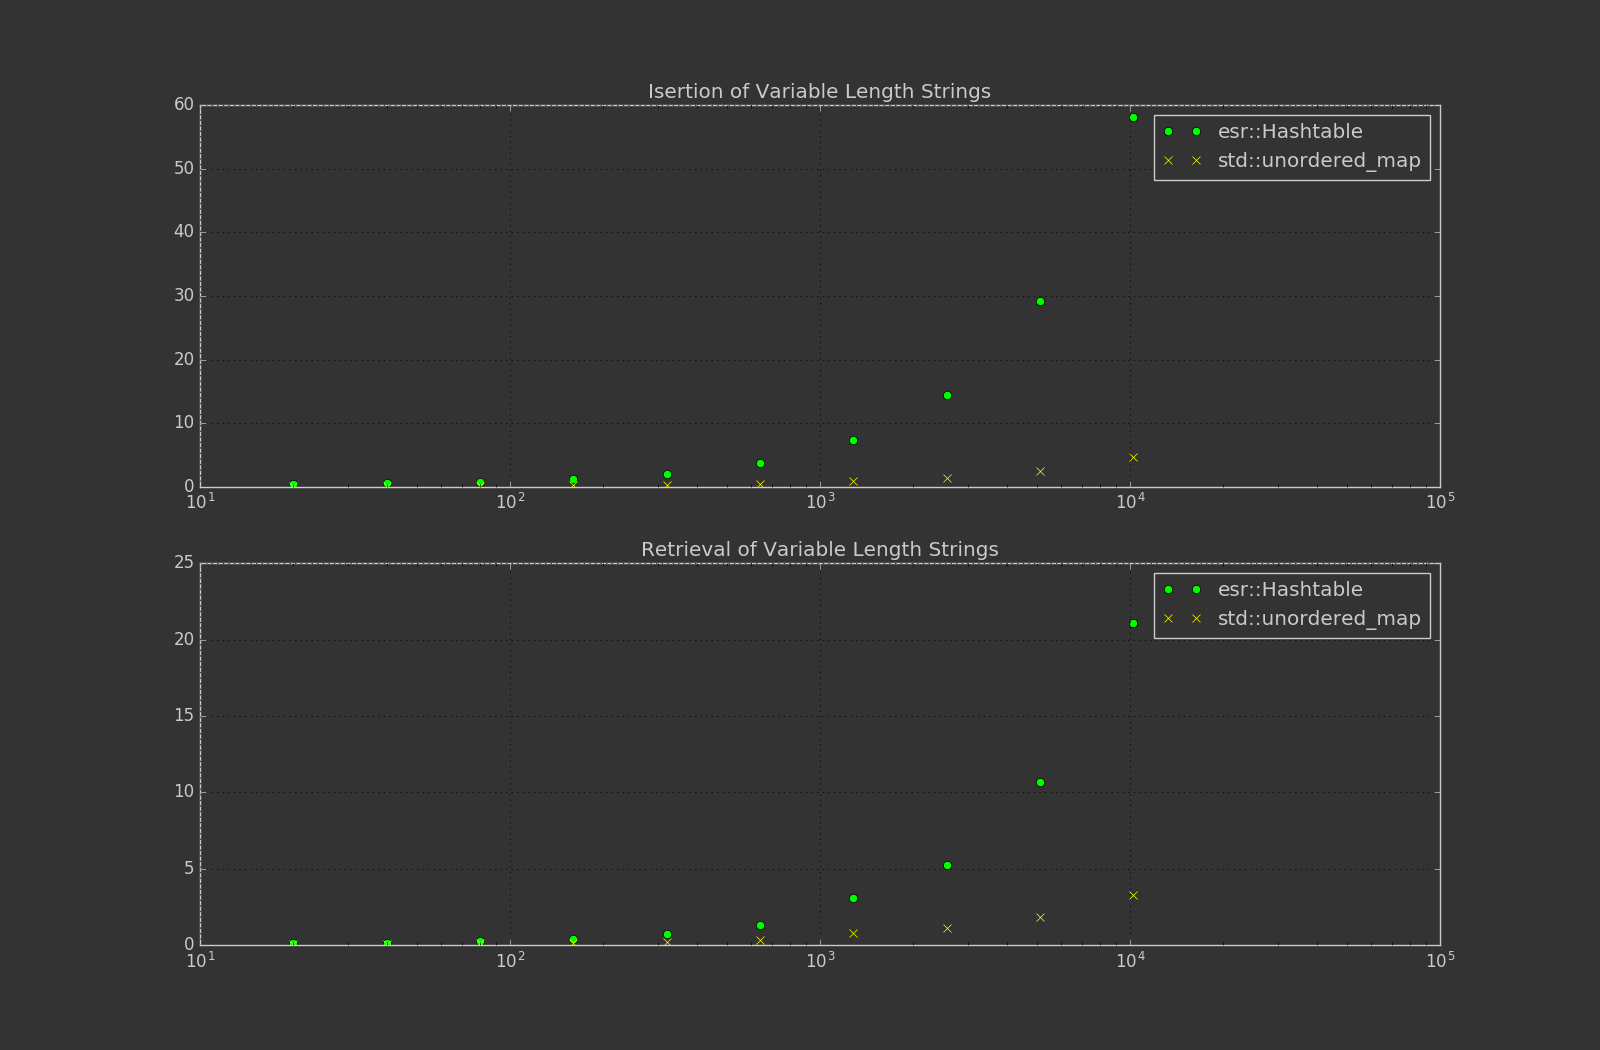
\includegraphics[scale=0.3]{vstr_perf}
  \end{figure}
\end{frame}


\begin{frame}{Tests.}{Performance. Summary.}
  \begin{table}[]
    \caption{Comparison of esr::Hashtable\footnote{ HT stands for esr::Hashtable.}
      and std::unordered\_map\footnote{ UM stands for std::unordered\_map.}. }
  
\label{my-label}

\centering
\resizebox{\textwidth}{!}{%
\begin{tabular}{lllll}
\hline
\textbf{OPERATION}    & \textbf{KEY TYPE} & \textbf{HT MEAN ($\mu$s)} & \textbf{UM MEAN ($\mu$s)} & \textbf{HT, UM DIFF ($\mu$s)}  \\ \midrule
\multirow{3}{*}{INSERTION} & integer           & 0.25437 & 0.22176  & 0.03261 \\
                           & fixed string      & 0.53371 & 0.30994  & 0.22375 \\
                           & var. string       & 11.78151 & 1.08067  & 10.70083 \\ \cmidrule(lr){2-5}
\multirow{3}{*}{RETRIEVAL} & integer           & 0.04087 & 0.04541  & 0.00454 \\
                           & fixed string      & 0.11612 & 0.05375  & 0.06236 \\
                           & var. string       & 4.30460 & 0.79793  & 3.50668 \\ \cmidrule(l){2-5} 
\end{tabular}%
}

\end{table}
\end{frame}

\begin{frame}{Tests.}{Application Sample.}
  Goal is to check Hashtable's functional correctness with custom type of keys and custom hash function.   
\end{frame}

\begin{frame}{Tests.}{Application Sample. Structure.}
  \begin{figure}
    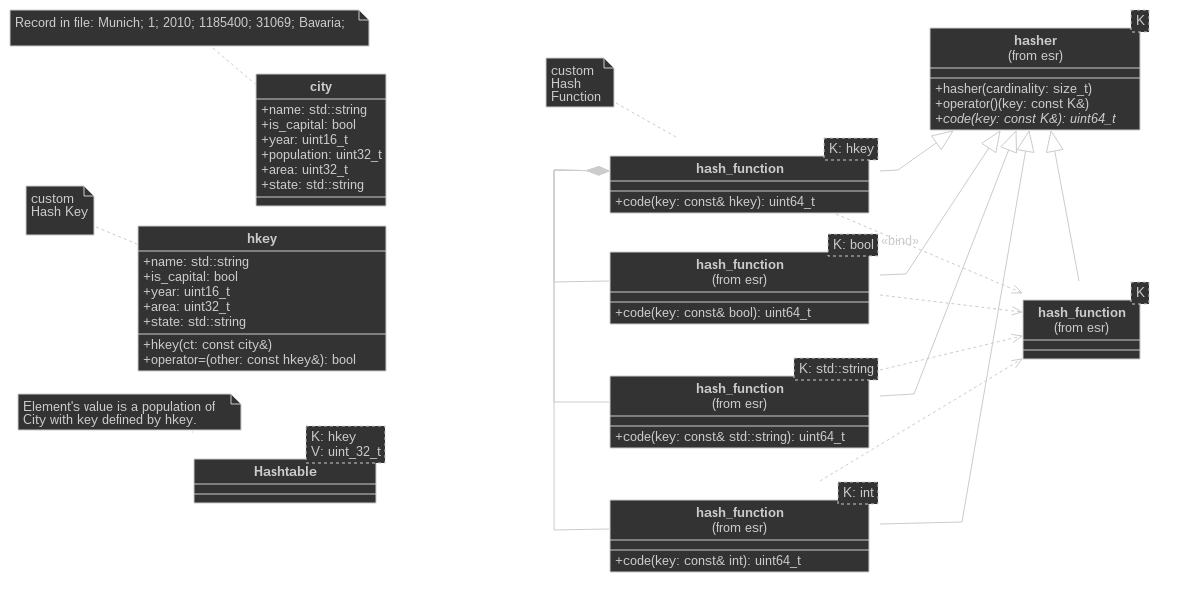
\includegraphics[scale=0.3]{structure_city_classes}
  \end{figure}
\end{frame}

\begin{frame}[fragile]{Tests.}{Application Sample. Custom Hash Function.}
\begin{lstlisting}[language=C++,basicstyle=\ttfamily\tiny,keywordstyle=\color{red}]
namespace esr {
  template <>
  class hash_function<city::hkey> : public esr::hasher<city::hkey> {
    public:
    explicit hash_function(size_t cardinality = 1, size_t start = 17, size_t prime = 31) :
                          esr::hasher<city::hkey>(cardinality),
                          m_bool_hasher(cardinality), m_int_hasher(cardinality),
                          m_string_hasher(cardinality),
                          m_start(start), m_prime(prime) {}

    uint64_t code(const city::hkey& key) const {
      uint64_t h = m_start;
      h = m_prime * h + m_bool_hasher.code(key.is_capital);
      h = m_prime * h + m_string_hasher.code(key.name);
      h = m_prime * h + m_int_hasher.code(key.year);
      h = m_prime * h + m_int_hasher.code(key.area);
      h = m_prime * h + m_string_hasher.code(key.state);
      return h;
    }

    private:
    size_t m_start;
    size_t m_prime;
    esr::hash_function<bool> m_bool_hasher;
    esr::hash_function<int> m_int_hasher;
    esr::hash_function<std::string> m_string_hasher;
  };
}  // namespace esr
\end{lstlisting}

\end{frame}

\section{Runtime Analysis.}

\begin{frame}{Runtime Analysis.}
  \begin{enumerate}
  \item Runtime estimation of INSERTION.
  \item Determenistic Hash Function vs. Universal Hash Funtion.
  \item Summary of runtime estimations for Hash Table's operations.
  \end{enumerate}
\end{frame}

%\begin{frame}{Runtime Analysis.}{Bucket.}
%  Bucket implemented as a Linked List.
%\begin{table}[]
%\centering
%\caption{Linked List Runtime.}
%\label{my-label}
%\begin{tabular}{@{}lll@{}}
%\toprule
%\textbf{operation} & \textbf{Big O} & \textbf{explaination}    \\ \midrule
%insertion          & O(n)           & scan for duplicated keys \\
%deletion           & O(n)           & scan list                \\
%find               & O(n)           & scan list                \\ \midrule
%front              & O(1)           & return first element     \\
%empty              & O(1)           & check first element      \\
%clear              & O(n)           & scan and delete elements \\ \bottomrule
%\end{tabular}
%\end{table}
%\end{frame}

\begin{frame}{Runtime Analysis.}{INSERTION. Naive.}
  Cost of insertion respective to input size is:
  \begin{equation}
    C^{insertion} = C^{hash} + C^{access} + C^{scan} + C^{create}
  \end{equation}
  \begin{equation} C^{hash} = O(1) \end{equation}
  \begin{equation} C^{access} = O(1) \end{equation}
  \begin{equation} \textcolor{orange}{C_{scan} = O(n)} \end{equation}
  \begin{equation} C^{create} = O(1) \end{equation}
  \begin{equation} C^{insertion} = O(n) \end{equation}
  Runtime is O(n) because of the $C^{scan}$.
  Bucket size should be constant, to perform $C^{scan}$ in O(1) time.
\end{frame}

\begin{frame}{Runtime Analysis.}{INSERTION with Resizing (I).}
  Load factor for $n$ elements in Hash Table and $m$ buckets is
  \begin{equation} \alpha = \frac{n}{m}.\end{equation}
  Expected size for an i'th bucket is
  \begin{equation} E[s_i] = \alpha. \end{equation}
  Hashtable is implemented as a Dynamic Array of buckets to maintain $\alpha$ in range from 0.5 to 1.
  Hashtable is expanded to it's double size when load factor is close to 1.
\end{frame}

\begin{frame}{Runtime Analysis.}{INSERTION with Resizing (II).}
  Cost of i'th insertion respective to input size is
  \begin{equation}
    C_i = H + A + S_i + V + R_i 
  \end{equation}
  \begin{equation}
    R_i = \begin{cases} (U + (A+(H+V)\cdot E[s_i])\cdot(i - 1), &\text{$\alpha$ $\geq$ 0.99}; \\
    0, & \text{otherwise}.
    \end{cases}
  \end{equation}
  Cost of resizing at i'th inserion  
  \begin{equation}
    R_i = \begin{cases} (U + (A+(H+V)\cdot\alpha)\cdot(i - 1), &\text{i-1 is a power of 2}; \\
    0, & \text{otherwise}.
    \end{cases}
  \end{equation}
  \begin{itemize}
  \item H is hash().
  \item A is access to bucket in array.
  \item S is scan bucket to find an element.
  \item V is cretaing an element and set key, value.
  \item U is creating new hash function.
  \end{itemize}
\end{frame}

\begin{frame}{Runtime Analysis.}{INSERTION with Resizing (III).}
  Amortized cost of insertion of n'th element is
  \begin{equation}
    C(n) = \frac{\sum_{i=1}^{n}C_i}{n} = \frac{(H+A+V)\cdot n}{n} + S(n) + R(n)
  \end{equation}
  Amortized cost of resizing at insertion of n'th element is
  \begin{equation}
    R(n) = \frac{\sum_{i=1}^{n)}R_i}{n} = \frac{n + \sum_{i=1}^{\log_2(n-1)}{(U+(A+(H+V)\cdot\alpha)\cdot2^i}}{n} 
  \end{equation}
  \begin{equation}
    R(n) = \left [\frac{log_2(n-1)}{n} \right ]\cdot U + \left [2-\frac{4}{n} \right ]\cdot (A+\alpha\cdot H + \alpha\cdot V) 
  \end{equation}
  Considering for load factor and bucket scan
  \begin{equation}
    \lim_{n \to \infty }\alpha= \lim_{n \to \infty }\left [\frac{n}{m} \right ] = \frac{1}{2},  
    \lim_{n \to \infty }S(n)= 1 
  \end{equation}
  Amortized cost of insertion
  \begin{equation}
    \lim_{n \to \infty }C(n)= 2\cdot H + 3\cdot A + 2\cdot V + 1 
  \end{equation}
  \begin{equation}
    O(2\cdot H)+O(3\cdot A)+O(2\cdot V)+O(1)=\color{yellow}O(1)
  \end{equation}
\end{frame}

\begin{frame}{Runtime Analysis.}{INSERTION with Resizing (IV).}
  \begin{figure}
    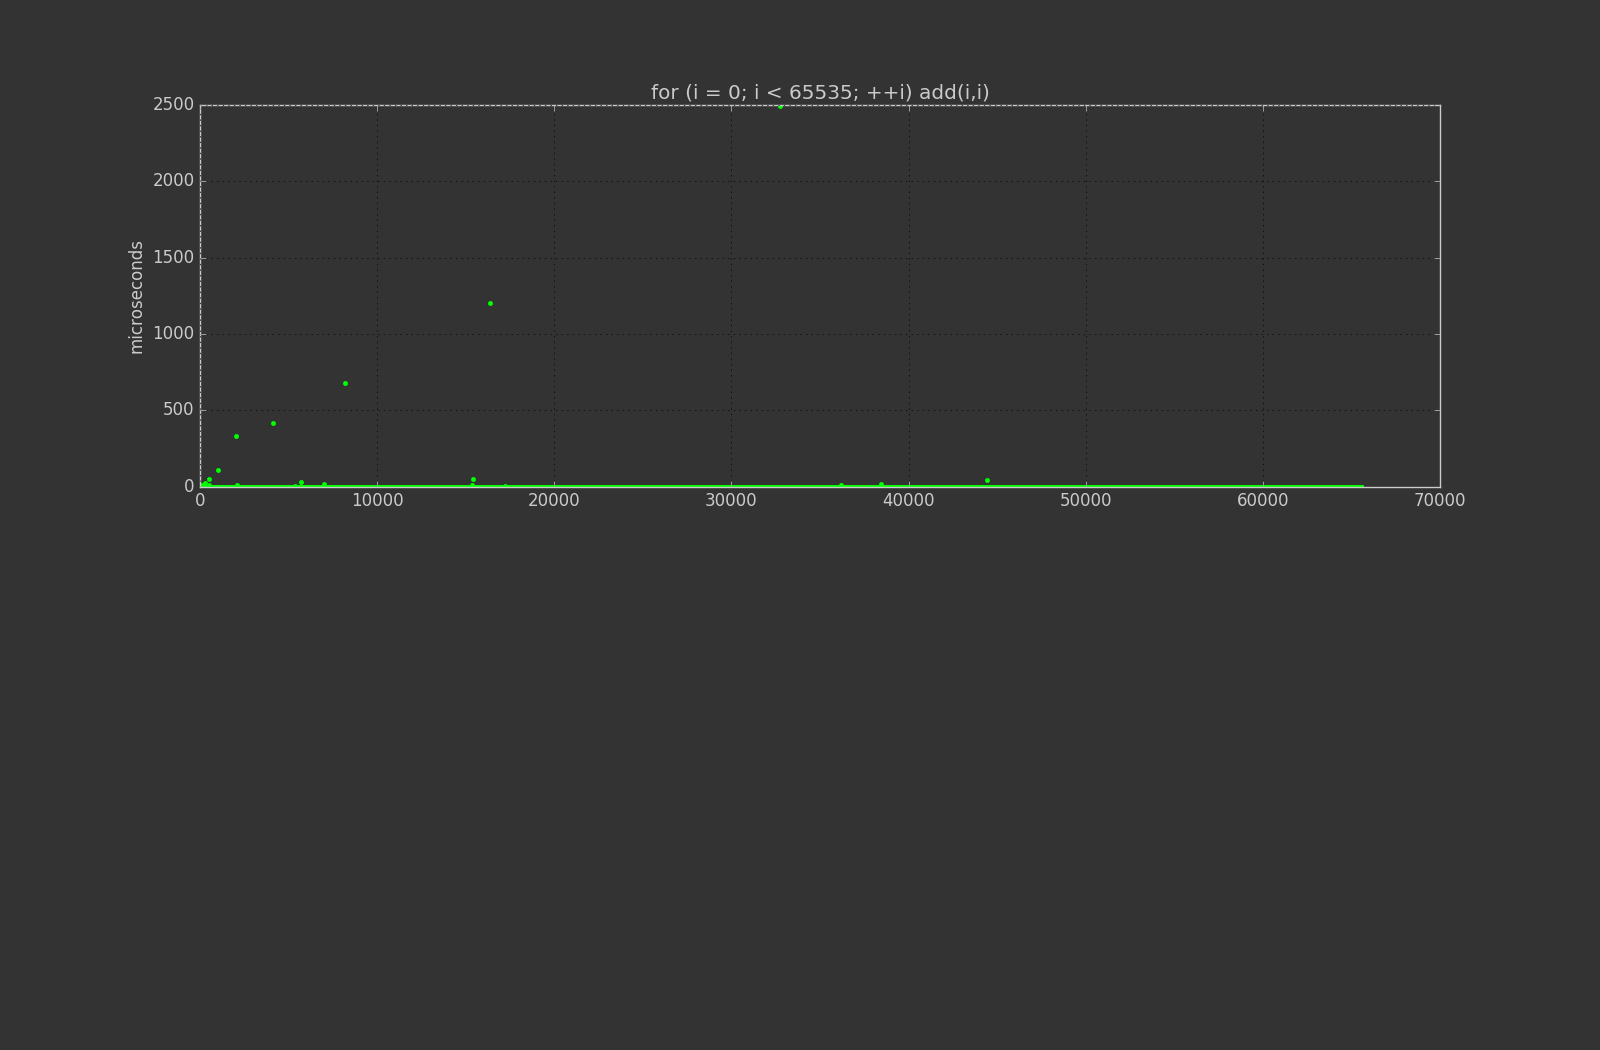
\includegraphics[scale=0.3]{insertion_amortized}
  \end{figure}
\end{frame}

  %%Expected bucket size is $E[n_i]$ = \alpha = n/m.
  %%Hashtable implemented as a Dynamic Array of Buckets to maintain \alpha in range 0.5 - 1.
  %%When n is close to 1 we expand an array by 2m.
  %%\framebreak

\begin{frame}{Runtime Analysis.}{Determenistic Hash Function.}
  \begin{itemize}
  \item For deterministic hash function, there is a bad input on which it will have a lot of collisions.
  \item Bad input is a powers of 2.
  \item Hash Table's content for maximum bad input size of 64 bit unsigned integer keys. 
  \end{itemize}
  \begin{figure}
    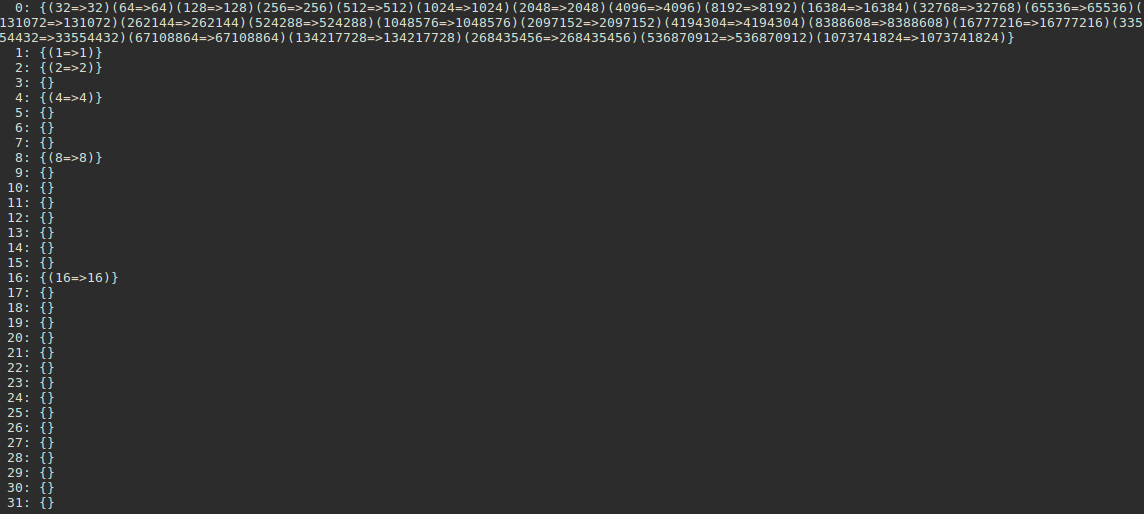
\includegraphics[scale=0.3]{worst_uint64_t_input}
  \end{figure}
\end{frame}

\begin{frame}{Runtime Analysis.}{Hash function from Universal Family.}
  \begin{itemize}
  \item Hash Fucntion selected from Universal Family of Hash Functions significantly resuces a number of collisions.
  \item Input is a powers of 2 is not bad one anymore.
  \item Hash Table's content for maximum bad input size of 64 bit unsigned integer keys. 
  \end{itemize}
  \begin{figure}
    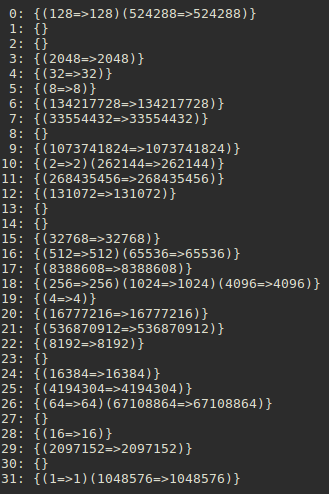
\includegraphics[scale=0.3]{uint64_t_universal}
  \end{figure}
\end{frame}

\begin{frame}{Tests.}{Performance. Hash Function for Integers.}
  \begin{table}[]
    \caption{Comparison of esr::Hashtable\footnote{ HT stands for esr::Hashtable.}
      and std::unordered\_map\footnote{ UM stands for std::unordered\_map.}. }
  
\label{my-label}

\centering
\resizebox{\textwidth}{!}{%
\begin{tabular}{lllll}
\hline
\textbf{OPERATION}    & \textbf{HASH FUNCTION} & \textbf{HT MEAN ($\mu$s)} & \textbf{UM MEAN ($\mu$s)} & \textbf{HT, UM DIFF ($\mu$s)}  \\ \midrule
\multirow{3}{*}{INSERTION} & Deterministic     & 0.29295 & 0.24536 & 0.04758 \\
                           & Universal         & 2.26267 & 0.24536 & 2.01731 \\ \cmidrule(lr){2-5}
\multirow{3}{*}{RETRIEVAL} & Deterministic     & 0.04228 & 0.05219 & 0.00991 \\
                           & Universal         & 0.22027 & 0.05219 & 0.16808 \\ \cmidrule(l){2-5}
\end{tabular}%
}

\end{table}
  esr::Hashtable's Universal/Deremenistic
  \begin{enumerate}
  \item INSERTION: 7.72367 times.
  \item RETRIEVAL: 5.20892 times.
  \end{enumerate}
\end{frame}




%%Total number
%%  of tests is 9*3*2 = 48, 9 is possible combinations of types, 3 is nuber
%%  of tested methods, 2 is positive and negative test. 
%%  tests for each of 3 functions.
  %Amortized cost = Cost(n operation) / n
  %respective to input size

\begin{frame}{Runtime Analysis.}{Summary.}
\begin{table}[]
\centering
\begin{tabular}{@{}lll@{}}
\toprule
\textbf{OPERATION} & \textbf{WORST} & \textbf{AMORTIZED} \\ \midrule
INSERTION          & O(n)           & O(1)               \\
DELETION           & O(n)           & O(1)               \\
FIND               & O(n)           & O(1)               \\
SET                & O(n)           & O(1)               \\
GET                & O(n)           & O(1)               \\
%%CREATE             & O(1)           & O(1)               \\
%%CREATE COPY        & O(n)           & O(n)               \\
%%ASSIGN             & O(n)           & O(n)               \\
%%DELETE             & O(n)           & O(n)               \\
ITERATOR BEGIN     & O(n)           & O(1)               \\
ITERATOR END       & O(1)           & O(1)               \\
ITERATOR ADVANCE   & O(n)           & O(1)               \\
ITERATOR COMPARE   & O(1)           & O(1)               \\
LOAD FACTOR        & O(1)           & O(1)               \\
SIZE               & O(1)           & O(1)               \\ \bottomrule
\end{tabular}
\caption{Runtime estimations for Hash Table's operations.}
\label{my-label}

\end{table}
\end{frame}

\begin{frame}{Conclusions.}{}
  Implemented Hash Table meets all requirements, performing all operation in O(1) amortized time.
  \par
  Delivarables
  \begin{itemize}
  \item Source Code.
  \item 15-minutes talk material.
  \end{itemize}
\end{frame}



\end{document}
